\input /users/davidmcallester/icloud/tex/SlidePreamble
\input /users/davidmcallester/icloud/tex/preamble

\begin{document}

{\Huge

  \centerline{\bf TTIC 31230, Fundamentals of Deep
  Learning} \bigskip \centerline{David McAllester, Autumn
  2023} \vfill \vfill \centerline{\bf Variational Auto-Encoders
  (VAEs)} \vfill \vfill

\slide{Generative AI: Autoregression and GANs}

A discrete autoregressive model can both generate samples and compute probabilities.

\vfill
This allows one to train a generative model by cross-entropy loss.

\vfill
But it is not obvious how to train a generative model of images by cross-entropy loss.

\vfill
{\color{red} The point of a VAE is to replace the adversarial loss of a GAN
with cross-entropy loss.}

\slide{Generative AI for Continuous Data: VAEs}
A variational autoencoder (VAE) is defined by three parts:

\vfill
\begin{itemize}
\item An encoder distribution $P_\enc(z|y)$.

\vfill
\item A ``prior'' distribution $P_\pri(z)$

\vfill
\item A generator distribution $P_\gen(y|z)$
\end{itemize}

\vfill
VAE generation uses $P_\pri(z)$ and $P_\gen(y|z)$ (like a GAN).

\vfill
VAE training uses a ``GAN inverter'' $P_\enc(z|y)$.

\slide{Fixed Encoder Training}
$$\pri^*,\gen^* = \argmin_{\pri,\gen}\;E_{y \sim \pop(y),z \sim \enc(z|y)}\left[-\ln P_\pri(z)P_\gen(y|z)\right]$$

\vfill
This is cross-entropy loss from $\pop(y)P_\enc(z|y)$ to $P_\pri(z)P_\gen(y|z)$

\vfill
Universality gives

{\color{red} $$P_{\pri^*}(z)P_{\gen^*}(y|z) = \pop(y)P_\enc(z|y)$$}

\vfill
Hence sampling from $P_{\pri^*}(z)P_{\gen^*}(y|z)$ samples $y$ from the population.


\slide{Training the Encoder (the GAN Inverter)}

Define the ELBO loss as follows (acronym described later).
\begin{eqnarray*}
{\cal L}(y,z) & = & - \ln \frac{P_\pri(z)P_\gen(y|z)}{P_\enc(z|y)}
\end{eqnarray*}

\begin{eqnarray*}
\enc^*,\pri^*,\gen^* & = & \argmin_{\enc,\pri,\gen}\;E_{\color{red} y \sim \pop,z\sim P_\enc(z|y)}\;{\cal L}(y,z)
\end{eqnarray*}

\vfill
For any encoder, universality gives

{\color{red} $$P_{\pri^*}(z)P_{\gen^*}(y|z) = \pop(y)P_\enc(y|z)$$}

\slide{Degrees of Freedom}

{\color{red} $$P_\pri(z)P_\gen(y|z) = \pop(y)P_\enc(z|y)$$}

\vfill
Any joint distribution on $(y,z)$ with the desired marginal on $y$ optimizes the bound.

\vfill
However, if we fix the architecture of $P_\pri(z)P_\gen(y|z)$ to be StyleGAN we can simultaneously train the parameters of the SyleGAN generator
and the StyleGAN inverter by cross-entropy loss.

\slide{Bayesian Interpretation}

VAEs were originally motivated by a Bayesian interpretation:

\vfill
\begin{itemize}
\item $P_\pri(z)$ is the Bayesian prior on hypothesis $z$.

\vfill
\item $P_\gen(y|z)$ is the propability of the ``evidence'' $y$ given hypothesis $z$.

\vfill
\item $P_\enc(z|y)$ is a model approximating the Bayesian posterior on hypothesis $z$ given evidence $y$.
\end{itemize}

\vfill
The Bayesian motivation is to train $P_\enc(z|y)$ to approximate Bayesian inference.

\slide{Bayesian Interpretation}
{\huge
\begin{eqnarray*}
\ln P_{\pri,\gen}(y) & =  & \ln \frac{P_{\pri,\gen}(y)P_{\pri,\gen}(z|y)}{P_{\pri,\gen}(z|y)} \\
\\
\\
& = & E_{z \sim P_\enc(z|y)}\left[\ln \frac{P_{\pri,\gen}(y)P_{\pri,\gen}(z|y)}{P_\enc(z|y)}\right] + KL(P_\enc(z|y),P_{\pri,\gen}(z|y)) \\
\\
\\
& \geq & E_{z \sim P_\enc(z|y)}\left[\ln \frac{P_{\pri,\gen}(y)P_{\pri,\gen}(z|y)}{P_\enc(z|y)}\right] \\
\end{eqnarray*}
}
A Bayesian thinks of $y$ as ``evidence'' for hypothesis $z$.

\vfill
{\color{red} $E_{z\sim P_\enc(z|y)}[-{\cal L}(y,z)]$} is called {\color{red} the evidence lower bound (ELBO)}.

\slide{Posterior Collapse}

Under the Bayesian interpretation we would like $z$ to provide useful information about (a causal origin of) $y$.

\vfill
However the objective function only produces
$$P_\pri(z)P_\gen(y|z) = \pop(y)P_\enc(z|y)$$

\vfill
For language models the generator can assign a meaningful probability to a block of text $y$ independent of $z$.

\vfill
When we train a sentence encoder (a thought vector) as the latent valriable of a language model VAE we can get a constant (zero) thought vector.

\vfill
This is called ``posterior collapse''.

\slide{The Reparameterization Trick}

$$\enc^* = \argmin_{\enc}\;\;E_{y\sim \pop(y),{\color{red} z\sim P_\enc(z|y)}}\;\left[- \ln \frac{P_\pri(z)P_\gen(y|z)}{P_\enc(z|y)}\right]$$

\vfill
Gradient descent on the encoder parameters must take into account the fact that we are sampling from the encoder.

\vfill
To handle this we sample noise $\epsilon$ from a fixed noise distribution and replace $z$ with a determinstc function $z_\enc(y,\epsilon)$

\vfill
$$\enc^*,\pri^*,\gen^* = \argmin_{\enc,\pri,\gen}\;\;E_{y,{\color{red} \epsilon,z=\hat{z}_\enc(y,\epsilon)}}\;\left[- \ln \frac{P_\pri(z)P_\gen(y|z)}{P_\enc(z|y)}\right]$$

\slide{The Reparameterization Trick}

$$\enc^*,\pri^*,\gen^* = \argmin_{\enc,\pri,\gen}\;\;E_{y,{\color{red} \epsilon,z=\hat{z}_\enc(y,\epsilon)}}\;\left[- \ln \frac{P_\pri(z)P_\gen(y|z)}{P_\enc(z|y)}\right]$$

\vfill
To get gradients we must have that $\hat{z}_\enc(y,\epsilon)$ is a differentiable function of the encoder parameters.

\vfill
Optimizing the encoder is tricky for discrete $z$.  Discrete $z$ is handled effectively in EM algorithms and general vector quantization (VQ) methods.

\slide{The KL-divergence Optimization}
\vfill
\begin{eqnarray*}
{\cal L}(y) & = & E_{z \sim P_\enc(z|y)}\left[ - \ln \frac{P_\pri(z)P_\gen(y|z)}{P_\enc(z|y)}\right] \\
\\
& = & {\color{red} KL(P_\enc(z|y),P_\pri(z))} + E_{z \sim P_\enc(z|y)}\left[- \ln P_\gen(y|z)\right] \\
\\
\\
&=& {\color{red} \frac{||\hat{z}_\enc(y) - \hat{z}_\pri||^2}{2\sigma^2}} + E_\epsilon\;\frac{||y - \hat{y}_\gen(\hat{z}_\enc(y,\epsilon))||^2}{2\sigma^2}
\end{eqnarray*}

\vfill
A closed-form expression for the KL term avoids sampling noise.

\slide{EM is Alternating Optimization of the ELBO Loss}

Expectation Maximimization (EM) applies in the (highly special) case where the exact posterior $P_{\pri,\gen}(z|y)$ is samplable and computable.
EM alternates exact optimization of $\enc$ and the pair $(\pri,\gen)$ in:
$$\mbox{VAE:}\;\;\;\;\;\;\; {\color{red} \pri^*,\gen^*} = \argmin_{\color{red} \pri,\gen} \min_{\color{red} \enc} E_{y,\;z \sim P_{\color{red} \enc}(z|y)}\;\;- \ln \frac{P_{\color{red} \pri,\gen}(z,y)}{P_{\color{red} \enc}(z|y)}$$

\vfill
$$\mbox{EM:}\;\;\;\;\;\; {\color{red} \pri^{t+1},\gen^{t+1}} =  \argmin_{\color{red} \pri,\gen}\;\;\;\;E_{y,\;z \sim P_{\color{red} \pri^t,\gen^t}(z|y)}\; - \ln P_{\color{red} \pri,\gen}(z,y)$$

\vfill
\centerline{\hspace{1em} Inference \hspace{6em} Update \hspace{2.5em}~}
\centerline{(E Step) \hspace{6em} (M Step) ~}
\centerline{ $P_\enc(z|y) = P_{\pri^{\color{red} t},\gen^{\color{red} t}}(z|y)$ \hspace{2.5em} Hold $P_\enc(z|y)$ fixed \hspace{0em}~}

\slide{Generative AI for Continuous Data: Flow Models}
$$\gen^* = \argmin_\gen \;E_{y \sim \popd(y)}\;-\ln p_\gen(y)$$

\vfill
Flow-based generative models work with Jacobians over continuous transformations (no ReLUs)
and can be directly trained with cross-entropy loss.

\vfill
But flow models have not caught on and we will not cover them.

\slide{Markovian VAEs}


\centerline{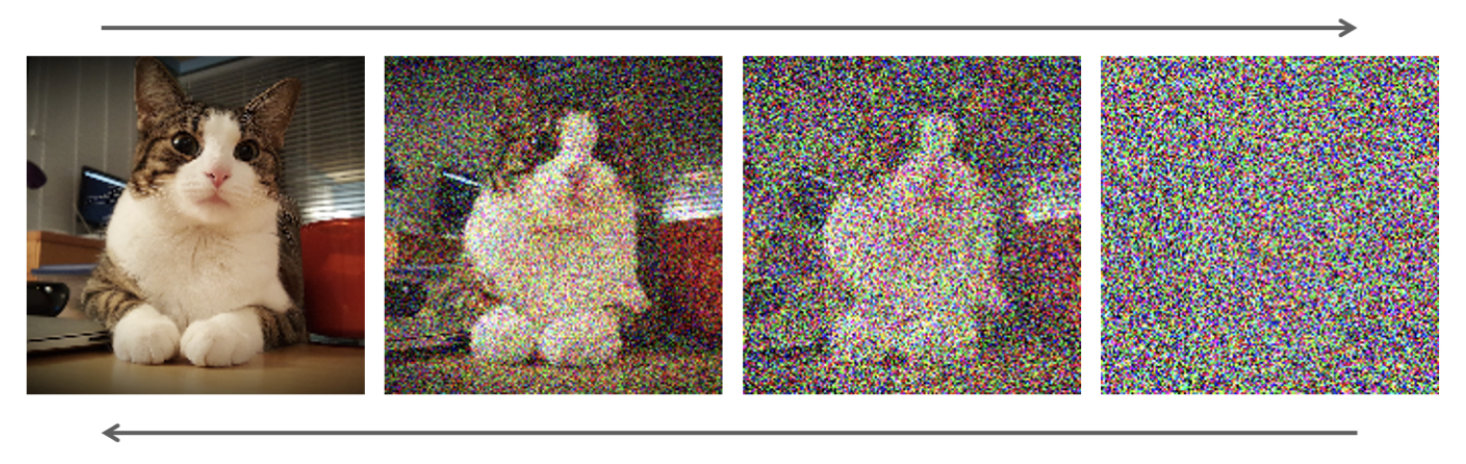
\includegraphics[width = 7in]{\images/DiffSequence}}

\vfill
{\huge
\centerline{{\color{red} [Sally talked to John]} $\stackrel{\rightarrow}{\leftarrow}$ {\color{red} [Sally talked to]}
$\stackrel{\rightarrow}{\leftarrow}$ {\color{red}[Sally talked]} $\stackrel{\rightarrow}{\leftarrow}$ {\color{red}[Sally]} $\stackrel{\rightarrow}{\leftarrow}$ {\color{red} []}}
}

\vfill
\centerline{$y \stackrel{\rightarrow}{\leftarrow} z_1  \stackrel{\rightarrow}{\leftarrow} \cdots \stackrel{\rightarrow}{\leftarrow} z_N$}

\slide{Markovian VAEs}
\centerline{$y \stackrel{\rightarrow}{\leftarrow} z_1  \stackrel{\rightarrow}{\leftarrow} \cdots \stackrel{\rightarrow}{\leftarrow} z_N$}

\vfill
{\bf Encoder}: $\pop(y)$, $P_\enc(z_1|y)$, and $P_\enc(z_{\ell+1}|z_\ell)$.


\vfill
{\bf Generator}: $P_\pri(z_N)$, $P_\gen(z_{\ell-1}|z_\ell)$, $P_\gen(y|z_1)$.

\vfill
The encoder and the decoder define distributions $P_\enc(y,\ldots,z_N)$ and $P_\gen(y,\ldots,z_N)$ respectively.


\slide{Markovian VAEs}

\centerline{$y \stackrel{\rightarrow}{\leftarrow} z_1  \stackrel{\rightarrow}{\leftarrow} \cdots \stackrel{\rightarrow}{\leftarrow} z_N$}

\vfill
\begin{itemize}
\item autoregressive models

\vfill
\item diffusion models

\vfill
\item Byte VAEs (original here)
\end{itemize}


\slide{Diffusion ELBO}

{\Large
\begin{eqnarray*}
H(y) & = & E_\enc\left[- \ln\frac{P_\enc(y)P_\enc(z_1,\ldots,z_N|y)}{P_\enc(z_1,\ldots,z_N|y)}\right]\\
  \\
  \\
  & = & E_\enc\left[ - \ln\frac{P_{\color{red} \enc}(y|z_1)P_{\color{red} \enc}(z_1|z_2)\cdots P_{\color{red} \enc}(z_{N-1}|z_N)P_{\color{red} \enc}(z_N)}
  {P_\enc(z_1|z_2,y)\cdots P_\enc(z_{N-1}|z_N,y)P_\enc(z_N|y)}\right] \\
   \\
   \\
  & {\color{red} \leq} & E_\enc\left[ - \ln\frac{P_{\color{red} \gen}(y|z_1)P_{\color{red} \gen}(z_1|z_2)\cdots P_{\color{red} \gen}(z_{N-1}|z_N)P_{\color{red} \gen}(z_N)}
  {P_\enc(z_1|z_2,y)\cdots P_\enc(z_{N-1}|z_N,y)P_\enc(z_N|y)}\right] \\
\\
\\
 & = & \left\{\begin{array}{l}E_\enc\;[-\ln P_\gen(y|z_1)]
                             \\ \\ + \sum_{i=2}^N  \; E_\enc\; KL(P_\enc(z_{i-1}|z_i,y),\;P_\gen(z_{i-1}|z_i)) \\
                             \\ + E_\enc\; KL(P_\enc(Z_N|y),p_\gen(Z_N))\end{array}\right.
\end{eqnarray*}
}

\slide{Byte VAEs}

A byte VAE is a numerical Markovian VAE with a deterministic encoder and where each $z_i$ is a vector of bytes.

\vfill
To computing $z_{i+1}(z_i)$ we first compute a floating point vector {\color{red} $\hat{z}^\enc_i(z_{i-1})$} and then round each coordinate to the nearest byte.

\vfill
We model  $-\ln P_\gen(z_i|z_{i+1})$ by {\color {red} $||\hat{z}^\enc_i(z_{i-1}) - \hat{z}^\gen_i(z_{i+1})||^2$}.

\vfill
Although the model is discrete, this gives gradients on both the encoder and the decoder.  This can be viewed as a straight-through gradient on the encoder.

\slide{The Byte VAE ELBO}

\begin{eqnarray*}
H(y) & \leq & E_{y\sim \pop}\left[- \ln\frac{P_\gen(z_N,z_{N-1},\ldots,z_1,y)}{P_\enc(z_1,\ldots,z_N|y)}\right]\\
\\
\\
& = & E_{y\sim \pop} [- \ln P_\gen(z_N,z_{N-1},\ldots,z_1,y)]
  \\
  \\
  & \approx & E_{y \sim \pop}\;\;{\color{red} ||y - \hat{y}^\gen(z_1)||^2 + \sum_{i=1}^{N-1} ||\hat{z}^\enc_i - \hat{z}^\gen_i(z_{i+1})||^2}
\end{eqnarray*}


\slide{END}

\end{document}
